\heading{理论力学-25春-期中1}

\begin{question}[圆盘的非完整约束]
一个半径为 $R$ 的均匀圆盘在二维平面 $x$--$y$ 上作无滑动纯滚动。设圆盘中心 $C$ 与圆盘和平面的接触点 $A$ 的连线 $CA$ 始终垂直于 $x$--$y$ 平面。分析系统的广义坐标与自由度，写出拉格朗日量 $L$，并用拉格朗日乘子法求广义坐标满足的微分方程。

\begin{solution}
圆盘始终竖直，故可取盘心坐标 $(x,y)$、圆盘前进方向角 $\varphi$ 和自转角 $\psi$ 为广义坐标。其中 $\varphi$ 是圆盘平面法线在 $xOy$ 平面内的方位角，$\psi$ 是绕圆盘对称轴的自转角。

均匀圆盘关于对称轴的转动惯量为
\[
  I_3=\frac12mR^2,
\]
关于任一直径的转动惯量为
\[
  I_1=\frac14mR^2.
\]
因此无约束形式的动能为
\[
  T=\frac12m(\dot x^2+\dot y^2)
    +\frac12 I_3\dot\psi^2+\frac12 I_1\dot\varphi^2
  =\frac12m(\dot x^2+\dot y^2)
    +\frac14mR^2\dot\psi^2+\frac18mR^2\dot\varphi^2 .
\]
势能为常数，可取为零，故 $L=T$。

纯滚动约束是接触点瞬时速度为零，即
\[
  \dot x=R\dot\psi\cos\varphi,
  \qquad
  \dot y=R\dot\psi\sin\varphi .
\]
这两个约束不可积分为仅含坐标的方程，因此系统有 $4$ 个广义坐标、$2$ 个独立非完整约束，运动自由度为
\ansmath{4-2=2.}

用拉格朗日乘子 $\lambda_1,\lambda_2$ 写约束为
\[
  \dot x-R\dot\psi\cos\varphi=0,
  \qquad
  \dot y-R\dot\psi\sin\varphi=0 .
\]
Lagrange--d'Alembert 方程为
\[
  m\ddot x=\lambda_1,
  \qquad
  m\ddot y=\lambda_2,
\]
\[
  \frac14mR^2\ddot\psi
  =-R(\lambda_1\cos\varphi+\lambda_2\sin\varphi),
  \qquad
  \frac14mR^2\ddot\varphi=0.
\]
连同两个约束方程共同决定系统运动。由最后一式可知
\ansmath{\dot\varphi=\text{const.}}
即圆盘前进方向的角速度保持不变。若先代入约束，则约化拉格朗日量为
\[
  L_{\mathrm{red} }
  =\frac34mR^2\dot\psi^2+\frac18mR^2\dot\varphi^2,
\]
但要强调：由于约束是非完整约束，严格推导运动方程应使用上面的乘子法，而不能把非完整约束当作完整约束直接变分。
\end{solution}

\end{question}

\begin{question}[匀质环与滑动质点]
一个质量为 $M$、半径为 $R$ 的均匀圆环，可绕通过环上一点且垂直于环面的水平轴自由转动。质量为 $m$ 的质点穿在圆环上，并可沿圆环无摩擦滑动。写出系统的拉格朗日方程，并求其在平衡位置附近的小振动解。

\begin{center}
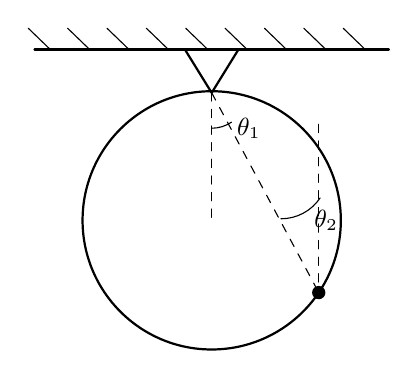
\begin{tikzpicture}[x=1cm,y=1cm,line cap=round,line join=round,font=\small]
  \draw[line width=0.8pt] (-2.25,2.05) -- (2.25,2.05);
  \foreach \x in {-2.05,-1.55,...,2.05} {\draw[thin] (\x,2.05) -- (\x-0.28,2.32);} 
  \coordinate (T) at (0,1.50);
  \draw[line width=0.8pt] (-0.34,2.05) -- (T);
  \draw[line width=0.8pt] (0.34,2.05) -- (T);
  \draw[line width=0.8pt] (0,-0.12) circle (1.64);
  \draw[dashed] (0,1.50) -- (0,-0.12);
  \coordinate (M) at ({1.64*cos(-34)},{1.64*sin(-34)-0.12});
  \draw[dashed] (T) -- (M);
  \draw[dashed] (1.36,1.10) -- (1.36,-1.12);
  \fill (M) circle (2.4pt);
  \draw (0.00,1.05) arc[start angle=-90,end angle=-56,radius=0.45];
  \node[right] at (0.20,1.05) {$\theta_1$};
  \draw (0.88,-0.10) arc[start angle=-90,end angle=-34,radius=0.60];
  \node[right] at (1.18,-0.12) {$\theta_2$};
\end{tikzpicture}

{\small 题 2 示意图}
\end{center}

\begin{solution}
设大环圆心相对悬点的方向角为 $\varphi$，质点相对大环圆心的绝对方向角为 $\psi$，二者均从竖直向下方向量起。大环关于悬点的转动惯量为
\[
  I_O=2MR^2.
\]
系统动能为
\[
  T=MR^2\dot\varphi^2+\frac12mR^2
  \left(\dot\varphi^2+\dot\psi^2+2\cos(\varphi-\psi)\dot\varphi\dot\psi\right),
\]
势能为
\[
  V=-(M+m)gR\cos\varphi-mgR\cos\psi.
\]
平衡位置附近的二次型为
\[
  T_2=\frac12R^2
  \begin{pmatrix}\dot\varphi&\dot\psi\end{pmatrix}
  \begin{pmatrix}2M+m&m\\m&m\end{pmatrix}
  \begin{pmatrix}\dot\varphi\\\dot\psi\end{pmatrix},
\]
\[
  V_2=\frac12gR
  \begin{pmatrix}\varphi&\psi\end{pmatrix}
  \begin{pmatrix}M+m&0\\0&m\end{pmatrix}
  \begin{pmatrix}\varphi\\\psi\end{pmatrix}.
\]
令 $\rho=M/m$，$\lambda=\omega^2R/g$，本征方程为
\[
  2\rho\lambda^2-(3\rho+2)\lambda+\rho+1=0.
\]
故
\[
  \boxed{\omega_1^2=\frac{g}{2R}},
  \qquad
  \boxed{\omega_2^2=\frac{M+m}{M}\frac{g}{R}}.
\]
模态可取为
\[
  \omega_1:\ \psi=\varphi,
  \qquad
  \omega_2:\ \psi=-\frac{M+m}{M}\varphi.
\]


\medskip
\textbf{本征方程细节：}线性化后系统满足
\[
  \mathbf M\ddot{\boldsymbol q}+\mathbf K\boldsymbol q=0,
  \qquad \boldsymbol q=(\varphi,\psi)^{\mathsf T},
\]
其中
\[
  \mathbf M=R^2\begin{pmatrix}2M+m&m\\m&m\end{pmatrix},
  \qquad
  \mathbf K=gR\begin{pmatrix}M+m&0\\0&m\end{pmatrix}.
\]
令 $\boldsymbol q=\boldsymbol a\ee^{\ii\omega t}$ 后求
\[
  \det(\mathbf K-\omega^2\mathbf M)=0.
\]
求出频率后再代回线性方程求振型，才能得到同相模态和反相模态。
\end{solution}
\end{question}

\begin{question}[滑环上二连杆系统的小振动]
一个质量为 $2m$ 的滑环可在光滑水平直杆上运动。两个质量均为 $m$ 的质点通过两根长度均为 $L$、质量可忽略的刚性轻杆依次悬挂在滑环下方，且重物的运动限制在同一竖直平面内。若两杆相对竖直方向的偏离都很小，求系统的小振动解。

\begin{center}
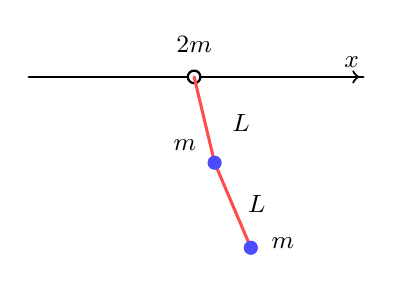
\begin{tikzpicture}[x=1cm,y=1cm,line cap=round,line join=round,font=\small]
  \draw[line width=0.8pt] (-2.10,1.15) -- (2.15,1.15);
  \draw[->,line width=0.8pt] (1.10,1.15) -- (2.10,1.15);
  \node[above] at (2.00,1.15) {$x$};
  \draw[line width=0.8pt,fill=white] (0,1.15) circle (0.08);
  \node[above] at (0,1.33) {$2m$};
  \coordinate (A) at (0,1.15);
  \coordinate (B) at (0.26,0.06);
  \coordinate (C) at (0.72,-1.02);
  \draw[line width=1.1pt,red!70] (A) -- (B) -- (C);
  \fill[blue!70] (B) circle (0.09);
  \fill[blue!70] (C) circle (0.09);
  \node[left] at (0.15,0.28) {$m$};
  \node[right] at (0.86,-0.96) {$m$};
  \node[right] at (0.36,0.56) {$L$};
  \node[right] at (0.56,-0.46) {$L$};
\end{tikzpicture}

{\small 题 3 示意图}
\end{center}

\begin{solution}
设滑环坐标为 $x$，两根轻杆相对竖直方向的小角分别为 $\theta_1,\theta_2$。保留二阶小量，两个质点的水平速度分别为
\[
  \dot x+L\dot\theta_1,
  \qquad
  \dot x+L\dot\theta_1+L\dot\theta_2.
\]
动能二次型为
\[
  T_2=m\dot x^2+\frac12m(\dot x+L\dot\theta_1)^2
  +\frac12m(\dot x+L\dot\theta_1+L\dot\theta_2)^2.
\]
势能二次型为
\[
  V_2=mgL\theta_1^2+\frac12mgL\theta_2^2.
\]
$x$ 为循环坐标。若初始总水平动量为零，则
\[
  4m\dot x+2mL\dot\theta_1+mL\dot\theta_2=0,
\]
即
\[
  \dot x=-\frac L4(2\dot\theta_1+\dot\theta_2).
\]
消去 $x$ 后，角变量的有效动能为
\[
  T_{\mathrm{eff}2}=\frac12mL^2
  \begin{pmatrix}\dot\theta_1&\dot\theta_2\end{pmatrix}
  \begin{pmatrix}1&1/2\\1/2&3/4\end{pmatrix}
  \begin{pmatrix}\dot\theta_1\\\dot\theta_2\end{pmatrix}.
\]
本征方程为
\[
  \det\left[
  \begin{pmatrix}2&0\\0&1\end{pmatrix}
  -\lambda\begin{pmatrix}1&1/2\\1/2&3/4\end{pmatrix}
  \right]=0,
  \qquad
  \lambda=\frac{\omega^2L}{g}.
\]
即
\[
  \lambda^2-5\lambda+4=0.
\]
故
\[
  \boxed{\omega_1=\sqrt{\frac gL}},
  \qquad
  \boxed{\omega_2=2\sqrt{\frac gL}}.
\]
对应模态为
\[
  \omega_1:\ \theta_2=2\theta_1,
  \qquad
  \omega_2:\ \theta_2=-\theta_1.
\]
系统小振动为二者线性叠加。
\end{solution}
\end{question}

\begin{question}[抛物线彗星的轨道时间]
某彗星在地球轨道平面内沿抛物线运动。设地球轨道为半径 $R$ 的圆，彗星轨道的近日点到太阳的距离为 $R/3$。求彗星位于地球轨道以内的时间（以年为单位）。

\begin{solution}
彗星在太阳引力场中作抛物线运动。设太阳引力参数为 $\mu=GM_\odot$，近日点距离为
\[
  q=\frac R3.
\]
抛物线轨道的半通径为
\[
  p=2q=\frac{2R}{3},
\]
轨道方程为
\[
  r=\frac{p}{1+\cos\nu},
\]
其中 $\nu$ 为真近点角。彗星位于地球轨道以内的边界由 $r=R$ 给出：
\[
  R=\frac{2R/3}{1+\cos\nu_0}
  \quad\Longrightarrow\quad
  \cos\nu_0=-\frac13.
\]
于是
\[
  \tan^2\frac{\nu_0}{2}
  =\frac{1-\cos\nu_0}{1+\cos\nu_0}=2,
  \qquad
  D_0=\tan\frac{\nu_0}{2}=\sqrt2 .
\]
抛物线运动的 Barker 公式为
\[
  t-t_p=\sqrt{\frac{2q^3}{\mu}}\left(D+\frac{D^3}{3}\right),
  \qquad D=\tan\frac\nu2 .
\]
从 $-\nu_0$ 到 $+\nu_0$ 的总时间为
\[
  \Delta t=2\sqrt{\frac{2q^3}{\mu}}
  \left(\sqrt2+\frac{(\sqrt2)^3}{3}\right)
  =\frac{20}{9\sqrt3}\sqrt{\frac{R^3}{\mu}}.
\]
地球公转周期为
\[
  T_E=2\pi\sqrt{\frac{R^3}{\mu}}.
\]
故以年为单位的时间为
\ansmath{\frac{\Delta t}{T_E}=\frac{10}{9\pi\sqrt3}\approx 0.204.}
也就是约 $0.204$ 年，约为 $74.5$ 天。


\medskip
\textbf{Barker 公式来源：}抛物线轨道满足 $e=1$，可引入
\[
  D=\tan\frac\nu2.
\]
由角动量守恒 $r^2\dot\nu=h$ 与抛物线参数 $p=h^2/\mu=2q$，可以把时间积分化为
\[
  t-t_p=\int_0^\nu \frac{r^2}{h}\,\dd\nu
  =\sqrt{\frac{2q^3}{\mu}}\left(D+\frac{D^3}{3}\right).
\]
由于进出地球轨道内侧的过程关于近日点对称，总时间必须取两倍。这也是结果中出现因子 $2$ 的原因。
\end{solution}

\end{question}

\begin{question}[四自由度系统的小振动]
一个自由度为 $4$ 的理想、完整且稳定约束的保守力学体系，其广义坐标为 $q_\alpha$（$\alpha=1,2,3,4$）。相应势能与动能二次型的系数矩阵分别为（设 $\omega_0>0$）
\[
  \mathbf{V}=\begin{pmatrix}
    1&0&0&0\\
    0&1&0&0\\
    0&0&2&-2\\
    0&0&-2&3
  \end{pmatrix}\omega_0^2,
  \qquad
  \mathbf{T}=\begin{pmatrix}
    1&0&0&0\\
    0&1&0&0\\
    0&0&1&-1\\
    0&0&-1&2
  \end{pmatrix}.
\]
\begin{enumerate}
  \item 求该体系的小振动解，并由求得的本征矢量判断哪些广义坐标已经是简正坐标；
  \item 找出全部简正坐标，并求其小振动解。
\end{enumerate}

\begin{solution}
小振动方程可写为
\[
  \mathbf T\ddot{\boldsymbol q}+\omega_0^2\mathbf V\boldsymbol q=0.
\]
令
\[
  \boldsymbol q=\boldsymbol a\ee^{\ii\omega t},
  \qquad
  \lambda=\frac{\omega^2}{\omega_0^2},
\]
得到广义本征值问题
\[
  (\mathbf V-\lambda\mathbf T)\boldsymbol a=0.
\]
直接计算
\[
  \det(\mathbf V-\lambda\mathbf T)=(\lambda-1)^3(\lambda-2).
\]
因此本征频率为
\ansmath{\omega=\omega_0\quad(\text{三重}),\qquad \omega=\sqrt2\,\omega_0\quad(\text{单重}).}
对应的本征矢量可取为
\[
  \lambda=1:
  \quad
  (1,0,0,0)^{\mathsf T},\quad
  (0,1,0,0)^{\mathsf T},\quad
  (0,0,1,1)^{\mathsf T},
\]
\[
  \lambda=2:
  \quad
  (0,0,1,0)^{\mathsf T}.
\]
\begin{enumerate}
  \item 由前两个本征矢量可见，$q_1$ 与 $q_2$ 本身已经是简正坐标；$q_3,q_4$ 的组合还需要重新选取。
  \item 按
  \[
    \boldsymbol q=Q_1(1,0,0,0)^{\mathsf T}
    +Q_2(0,1,0,0)^{\mathsf T}
    +Q_3(0,0,1,1)^{\mathsf T}
    +Q_4(0,0,1,0)^{\mathsf T}
  \]
  展开，可得
  \[
    q_1=Q_1,
    \qquad
    q_2=Q_2,
    \qquad
    q_3=Q_3+Q_4,
    \qquad
    q_4=Q_3.
  \]
  因而一组简正坐标为
  \ansmath{Q_1=q_1,
    \qquad Q_2=q_2,
    \qquad Q_3=q_4,
    \qquad Q_4=q_3-q_4.}
  它们满足
  \[
    \ddot Q_1+\omega_0^2Q_1=0,
    \quad
    \ddot Q_2+\omega_0^2Q_2=0,
    \quad
    \ddot Q_3+\omega_0^2Q_3=0,
  \]
  \[
    \ddot Q_4+2\omega_0^2Q_4=0.
  \]
  所以
  \[
    Q_j=A_j\cos(\omega_jt)+B_j\sin(\omega_jt),
  \]
  其中 $\omega_1=\omega_2=\omega_3=\omega_0$，$\omega_4=\sqrt2\omega_0$。
  \item 简并频率为 $\omega_0$，简并度为 $3$；频率 $\sqrt2\omega_0$ 不简并。
\end{enumerate}
\end{solution}

\end{question}

\begin{question}[Yukawa 核力势中的圆运动]
根据 Yukawa 核力理论，中子与质子之间的吸引势能为
\[
  V(r)=-\frac{k\ee^{-\alpha_0 r}}{r},
  \qquad k>0,\quad \alpha_0>0.
\]
求质量为 $m$ 的粒子在该势场中作半径为 $a$ 的圆周运动时的能量 $E$ 和角动量 $J$，并讨论该圆周运动的稳定性条件。

\begin{solution}
有效势能为
\[
  V_{\mathrm{eff}}(r)=\frac{J^2}{2mr^2}-\frac{k\ee^{-\alpha_0r}}{r}.
\]
半径为 $a$ 的圆运动满足
\[
  V_{\mathrm{eff}}'(a)=0.
\]
由此得
\[
  \boxed{J^2=mka\ee^{-\alpha_0a}(1+\alpha_0a)}.
\]
圆运动的能量为
\[
  E=\frac{J^2}{2ma^2}-\frac{k\ee^{-\alpha_0a}}{a}
  =\boxed{\frac{k\ee^{-\alpha_0a}}{2a}(\alpha_0a-1)}.
\]
稳定性要求
\[
  V_{\mathrm{eff}}''(a)>0.
\]
计算得
\[
  V_{\mathrm{eff}}''(a)=\frac{k\ee^{-\alpha_0a}}{a^3}
  \left(1+\alpha_0a-\alpha_0^2a^2\right).
\]
故稳定条件为
\[
  \boxed{1+\alpha_0a-\alpha_0^2a^2>0}
  \quad\Longleftrightarrow\quad
  \boxed{0<\alpha_0a<\frac{1+\sqrt5}{2}}.
\]


\medskip
\textbf{关键步骤：}也可由向心力方程验证角动量表达式。势能给出的径向力为
\[
  F_r=-\frac{\dd V}{\dd r}
  =-k\ee^{-\alpha_0r}\left(\frac{\alpha_0}{r}+\frac{1}{r^2}\right).
\]
半径为 $a$ 的圆周运动满足
\[
  \frac{mv^2}{a}=k\ee^{-\alpha_0a}\left(\frac{\alpha_0}{a}+\frac{1}{a^2}\right),
\]
于是
\[
  J=mav,
  \qquad
  J^2=mka\ee^{-\alpha_0a}(1+\alpha_0a),
\]
与有效势法一致。能量中的动能项为 $J^2/(2ma^2)$，代入后才能得到 $E$；不要把势能本身误认为总能量。
\end{solution}
\end{question}

\begin{question}[硬球弹性碰撞的散射截面]
两个质量均为 $m$、半径均为 $R$ 的硬球发生弹性碰撞。球 $A$ 在实验室参考系中静止，球 $B$ 从远处以初速度 $v_0$ 入射，碰撞参数为 $b$。求实验室参考系中的微分散射截面 $\dd\sigma/\dd\Omega$ 和总散射截面 $\sigma$。

\begin{solution}
两个等质量硬球的弹性碰撞可化为相对运动问题：一个约化粒子被半径
\[
  a=2R
\]
的硬球散射。质心系中硬球散射的关系为
\[
  b=a\cos\frac\chi2,
\]
其中 $\chi$ 是质心系散射角。因此
\[
  \frac{\dd\sigma}{\dd\Omega_{\mathrm{cm}}}
  =\frac{b}{\sin\chi}\left|\frac{\dd b}{\dd\chi}\right|
  =\frac{a^2}{4}=R^2.
\]
总截面为
\[
  \boxed{\sigma=\pi a^2=4\pi R^2}.
\]
对实验室系中入射球的散射角 $\theta$，等质量弹性碰撞给出
\[
  \chi=2\theta,
  \qquad 0\le\theta\le\frac\pi2.
\]
又
\[
  \dd\Omega_{\mathrm{cm}}=4\cos\theta\,\dd\Omega_{\mathrm{lab}}.
\]
故实验室系中入射球的微分截面为
\[
  \boxed{\frac{\dd\sigma}{\dd\Omega_{\mathrm{lab}}}
  =4R^2\cos\theta,
  \qquad 0\le\theta\le\frac\pi2.}
\]
对该式在实验室半球积分，仍得 $4\pi R^2$。


\medskip
\textbf{实验室系转换细节：}等质量弹性碰撞中，入射球在实验室系的散射角 $\theta$ 与质心系相对速度的散射角 $\chi$ 满足
\[
  \theta=\frac{\chi}{2}.
\]
立体角元满足
\[
  \dd\Omega_{\mathrm{cm}}=2\pi\sin\chi\,\dd\chi
  =2\pi\sin(2\theta)\,2\dd\theta
  =4\cos\theta\,\dd\Omega_{\mathrm{lab}}.
\]
因此从质心系常数截面 $a^2/4$ 到实验室系时必须乘上这个 Jacobian。实验室系中入射球只散射到前半球，故 $0\le\theta\le\pi/2$。


\medskip
硬球散射关系 $b=a\cos(\chi/2)$ 来自几何反射。入射相对速度沿直线接近半径为 $a$ 的硬球，最近点处法线与入射方向的夹角满足 $\sin\beta=b/a$，反射使速度方向转过 $\chi=\pi-2\beta$，故
\[
  b=a\sin\beta=a\cos\frac\chi2.
\]
因此截面完全由几何半径决定，与入射速度 $v_0$ 无关；$v_0$ 只影响碰撞后的速度大小和时间尺度。
\end{solution}
\end{question}
